% !TEX TS-program = pdflatex
% !TEX encoding = UTF-8 Unicode

% This is a simple template for a LaTeX document using the "article" class.
% See "book", "report", "letter" for other types of document.

\documentclass[11pt]{article} % use larger type; default would be 10pt

\usepackage[utf8]{inputenc} % set input encoding (not needed with XeLaTeX)

%%% Examples of Article customizations
% These packages are optional, depending whether you want the features they provide.
% See the LaTeX Companion or other references for full information.

%%% PAGE DIMENSIONS
\usepackage{geometry} % to change the page dimensions
\geometry{a4paper} % or letterpaper (US) or a5paper or....
% \geometry{margin=2in} % for example, change the margins to 2 inches all round
% \geometry{landscape} % set up the page for landscape
%   read geometry.pdf for detailed page layout information

\usepackage{graphicx} % support the \includegraphics command and options

% \usepackage[parfill]{parskip} % Activate to begin paragraphs with an empty line rather than an indent

%%% PACKAGES
\usepackage{booktabs} % for much better looking tables
\usepackage{array} % for better arrays (eg matrices) in maths
\usepackage{paralist} % very flexible & customisable lists (eg. enumerate/itemize, etc.)
\usepackage{verbatim} % adds environment for commenting out blocks of text & for better verbatim
\usepackage{subfig} % make it possible to include more than one captioned figure/table in a single float
% These packages are all incorporated in the memoir class to one degree or another...

%%% HEADERS & FOOTERS
\usepackage{fancyhdr} % This should be set AFTER setting up the page geometry
\pagestyle{fancy} % options: empty , plain , fancy
\renewcommand{\headrulewidth}{0pt} % customise the layout...
\lhead{}\chead{}\rhead{}
\lfoot{}\cfoot{\thepage}\rfoot{}

%%% SECTION TITLE APPEARANCE
\usepackage{sectsty}
\allsectionsfont{\sffamily\mdseries\upshape} % (See the fntguide.pdf for font help)
% (This matches ConTeXt defaults)

%%% ToC (table of contents) APPEARANCE
\usepackage[nottoc,notlof,notlot]{tocbibind} % Put the bibliography in the ToC
\usepackage[titles,subfigure]{tocloft} % Alter the style of the Table of Contents
\renewcommand{\cftsecfont}{\rmfamily\mdseries\upshape}
\renewcommand{\cftsecpagefont}{\rmfamily\mdseries\upshape} % No bold!

\usepackage{amsmath}
\usepackage{amsfonts}
%\usepackage{mathcal}

% Pseudocode
\usepackage[]{algorithm}
\usepackage{algpseudocode}[noend]

%%% END Article customizations

%%% The "real" document content comes below...

\title{Project 1 in FYS3150}
\author{Simon Halstensen, Carl Fredrik Nordbø Knutsen, Jan Harald Aasen \& Didrik Sten Ingebrigtsen}
\date{05.09.2021} % Activate to display a given date or no date (if empty),
         % otherwise the current date is printed 

\begin{document}
\maketitle
In this project we are solving the following equation:
\begin{equation} - \dfrac{d^2u}{dx^2} = f(x) \end{equation}
We also know that:
\begin{itemize}
	\item \(f(x) = 100e^{-10x}\)
	\item \(x \in [0, 1]\)
	\item \(u(0)=u(1)=0\)
\end{itemize}

\section*{Exercise 1}


I will check that 
\begin{equation}  u(x) = 1 - (1- e^{-10})x -e^{-10x} \end{equation}
is a solution to (1) by differentiating \(u(x)\) twice. 

\[\dfrac{d^2u}{dx^2} =\dfrac{d}{dx}(\dfrac{du}{dx}) = \dfrac{d}{dx}( -(1 - e^{-10}) - (-10)e^{-10x})\]
And since the derivative of a constant is 0, we get that: 
\[\dfrac{d^2u}{dx^2} = \dfrac{d}{dx}(10e^{-10x}) = -100e^{-10x}\]
It immediately follows that
\[ - \dfrac{d^2u}{dx^2} = 100e^{-10x}\]
This shows that (2) is a solution to equation (1).
This solution also satisfies the boundary conditions specified, as:
\[u(0) = 1 - (1- e^{-10})0 -e^{-10\cdot 0} = 1-1 = 0\]
and
\[u(1) = 1 - (1- e^{-10})1 -e^{-10\cdot 1} = 0\]

\section*{Exercise 2}

The program main.cpp evaluates the exact function \(u(x)\) from exercise 1, at points between 0 and 1. 
It writes the \(x\)-values and \(u(x)\)-values to a .csv-file, named exact\_evaluated.csv.
The python script read\_file\_and\_plot.py reads the values from the .csv-file, and plots the function (see figure 1).
\begin{figure}[htbp]
\centerline{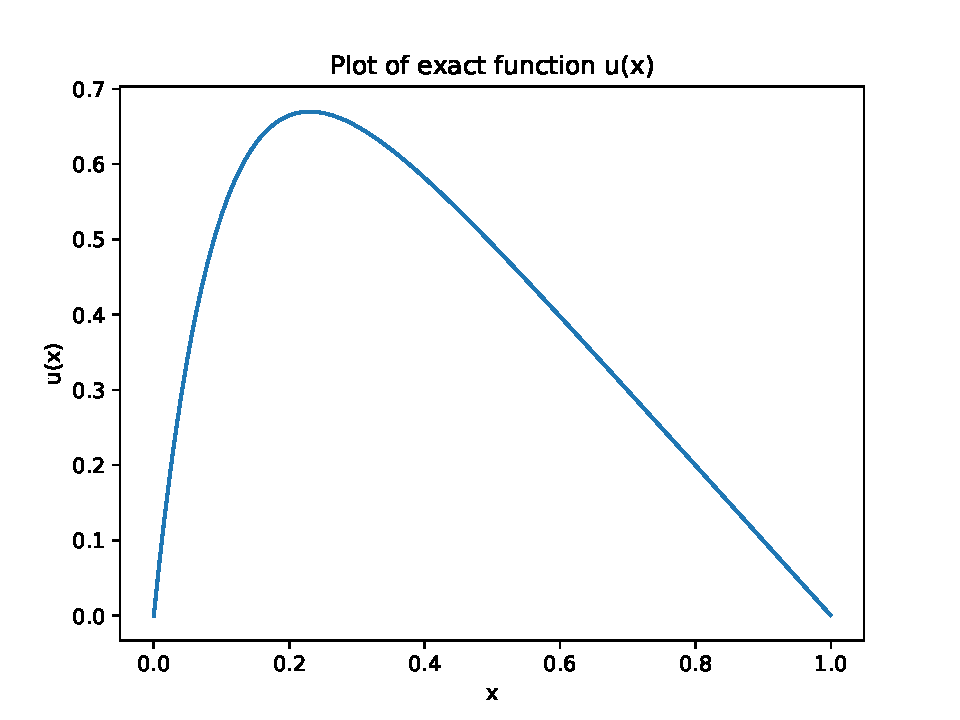
\includegraphics{exact_function_u(x).pdf}}
\caption{Plot of the exact function \(u(x) = 1 - (1- e^{-10})x -e^{-10x}\)}
\label{fig}
\end{figure}

\section*{Exercise 3}

I will derive a discretized version of equation (1) by finding a discretized approximation of \(\dfrac{d^2u}{dx^2}=u''(x)\).  
Let \(h\) be a step size, and let \(a\) be a point such that \(a \in [h, 1-h]\). Firstly, evaluate the 3rd degree Taylor expansion of u(x) about the point \(a\) in the points \(a+h\) and \(a-h\).
\[u(a+h) =u(a) + u'(a)\cdot h + \dfrac{1}{2}u''(a) \cdot h^2 + \dfrac{1}{6}u'''(a) \cdot h^3 + \mathcal{O}(h^4) \]
\[u(a-h) =u(a) + u'(a)\cdot (-h) + \dfrac{1}{2}u''(a) \cdot h^2 + \dfrac{1}{6}u'''(a) \cdot (-h)^3 + \mathcal{O}(h^4) \]
Next, add the two equations, giving the following equality.
\[ u(a+h) + u(a-h) = 2u(a) + u''(a)\cdot h^2 + \mathcal{O}(h^4) \]
The equation can be solved for \(u''(a)\)
\[u''(a) = \dfrac{u(a+h) - 2u(a) +u(a-h)}{h^2} + \mathcal{O}(h^2) \]
Assuming a sufficiently small value for h, we can approximate and discretize with \(u(ih) \approx v_i\). Here, \(i \in \{0, 1, .., n\}\) (meaning \(n=\dfrac{1}{h}\)), and:
\[u''(ih) = \dfrac{v_{i+1} - 2v_i +v_{i-1}}{h^2} \]
Using equation (1), we can rewrite:
\begin{equation}h^2 \cdot f(ih) = -v_{i+1} + 2v_i - v_{i-1}\end{equation}
Which is a discretized version of equation (1) with the following conditions:
\begin{itemize}
	\item \(v_0=u(0)=0\) 
	\item \(v_{n}=u(1)=0\).
\end{itemize}

\section*{Exercise 6}

\subsection*{a)}

In this exercise, we want to formulate the algorithm for solving $Ax = g$ for a general tridiagonal $A$. This is done in [alg \ref{alg:general}].

\begin{algorithm}
\caption{Algorithm for solving $Ax = g$ for a general tridiagonal matrix $A$. $a$, $b$ and $c$ represent the sub-, main- and superdiagonal. Solving it means taking in $A$ and $g$, and returning $x$.}
\begin{algorithmic}[0]
\Procedure{tridiagonal solver}{a, b, c, g, N}
    \State $\tilde{b}_0 \gets b_0$
    \State $\tilde{g}_0 \gets g_0$
    \For{$i \in (1, N)_{\mathbb{N}}$}
        \State $\tilde{b}_i \gets b_i - \frac{a_i}{\tilde{b}_{i-1}} c_{i-1}$
        \State $\tilde{g}_i \gets g_i - \frac{a_i}{\tilde{b}_{i-1}} \tilde{g}_{i-1}$
    \EndFor
    \State $x_N \gets \frac{\tilde{g}_N}{\tilde{b}_N}$
    \For{$i \in (N-1, 0)_{\mathbb{N}}$}
        \State $x_i \gets \frac{\tilde{g}_i - c_i x_{i+1}}{\tilde{b}_i}$
    \EndFor
    \State \Return $x$
\EndProcedure
\end{algorithmic}
\label{alg:general}
\end{algorithm}

\subsection*{b)}
The number of floating point operations (FLOPs) in the general algorithm in [alg \ref{alg:general}] is $2 \cdot 3 N = 6N$, where $N$ is the size of the matrix, for forward substitution. For back substitution, we have $3 N$ FLOPs. In total, the algorithm has $9N = \mathcal{O}(N)$ FLOPs. 


\end{document}
